\chapter{Исследовательская часть}

\section{Технические характеристики}
Технические характеристики устройства, на котором выполнялись
замеры по времени:

\begin{itemize}
    \item Процессор: Intel Core i7 9750H 2.6 ГГц;
    \item Оперативная память: 16 ГБ;
    \item Операционная система: Kubuntu 22.04.3 LTS x86\_64 Kernel: 6.2.0-36-generic
\end{itemize}

Во время проведения измерений времени ноутбук был подключен к сети электропитания и был нагружен только системными приложениями.

\section{Демонстрация работы программы}

На рисунке \ref{fig:img_prog} показан пример работы с программой.


\begin{figure}[ht!]
	\centering
	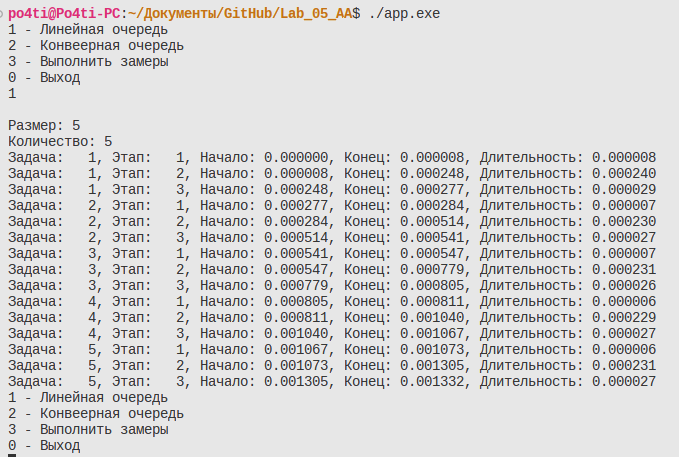
\includegraphics[width=170mm]{img/img_prog.png}
	\caption{Демонстрация работы программы.\label{overflow}}
	\label{fig:img_prog}
	\end{figure}


\clearpage

\section{Временные характеристики}


Исследование временных характеристик реализованных алгоритмов производилось на массивах размером 1 -- 8 с шагом 1.

\begin{figure}[ht!]
	\centering
	\includesvg[width=1.0\textwidth]{inc/img/plotting_data1.svg}
	\caption{Результат измерений времени работы (в мс) алгоритмов при разных размерах матриц\label{overflow}}
	\label{fig:plotting_data1}
	\end{figure}
\clearpage

\begin{figure}[ht!]
	\centering
	\includesvg[width=1.0\textwidth]{inc/img/plotting_data2.svg}
	\caption{Результат измерений времени работы (в мс) алгоритмов при разном кол-ве матриц\label{overflow}}
	\label{fig:plotting_data2}
	\end{figure}


% \addcontentsline{toc}{section}{Вывод}
\section{Вывод}

При разных размерах матриц, в связи с разной сложностью заявок, при больших размерах матриц возникает проблема горлышка бутылки. Из-за экспоненциального роста второй заявки разница между конвеерным и линейным алгоритмом стремится к нулю.

При одинаковых размерах матриц, конвеерная обработка заявок занимает меньше времени, чем линейная обработка.